\chapter{Desarrollo del Hardware} \label{ch:development}

% **************************** Define Graphics Path **************************
\ifpdf
    \graphicspath{{Chapter3/Figs/Raster/}{Chapter3/Figs/PDF/}{Chapter3/Figs/}}
\else
    \graphicspath{{Chapter3/Figs/Vector/}{Chapter3/Figs/}}
\fi

En este capítulo se presenta el desarrollo físico del dispositivo en función de las bases teóricas y los requerimientos definidos en el capítulo previo. El mismo se encuentra dividido en dos secciones. En la primera se explica que criterios fueron tomados en cuenta y que componentes se utilizaron para la construcción de cada sección del radar. En la segunda, se muestran las mediciones realizadas para caracterizar los distintos módulos que lo integran.


\section{Construcción}

En la figura \ref{fig:radarDiagram} se puede observar un diagrama en bloques mostrando los distintos módulos que integran el radar construido. Las siguientes secciones del capítulo explican cada uno de estos módulos por separado, salvo el procesador que se explicará en el capítulo \ref{sc:radarProcessor}.
\begin{figure}
 \centering
 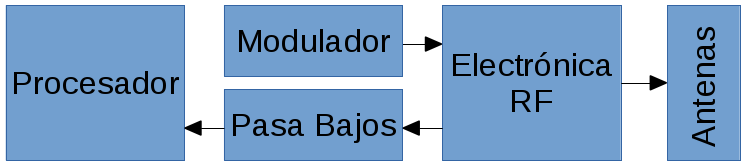
\includegraphics[width=10cm]{radarScheme}
 \caption{Diagrama en bloques básico del radar FMCW a construir.}
 \label{fig:radarDiagram}
\end{figure}


\subsection{Modulador}

Como se mencionó en la sección \ref{sc:ambiguity}, para evitar ambigüedades en la determinación del rango de medición la duración de la chirp transmitida debe ser mayor que el tiempo de ida y vuelta al blanco más alejado detectable por el radar. Como se desea una distancia máxima igual a $\SI{20}{\meter}$ (ver requerimiento \ref{req:l0}), siguiendo la relación de la ecuación \ref{eq:relDist}, se puede determinar el mínimo valor admitido de dicho período.
\begin{equation}
  \tau = \dfrac{2R\sqrt{\varepsilon_r}}{c} \approx \SI{133.43}{\nano\second}
\end{equation}

A su vez, en la sección \ref{sc:ambiguity} también se mencionó que para disminuir errores en el cálculo de la estimación en la frecuencia, se busca que el período de la señal transmitida sea al menos dos órdenes mayor que el máximo tiempo de ida y vuelta. Por lo tanto, el mínimo período resulta igual a $\SI{13.343}{\mu\second}$. De esta forma se desprende el requerimiento \ref{req:l2_pulseT}.

Las especificaciones del modulador utilizado en todos los ensayos están definidos en la tabla \ref{tab:modulatorsSpecification}. Las mismas definen los requerimientos \ref{req:l2_mod} y \ref{req:l2_dutyCycle}.

\begin{table}[htb]
  \caption{Especificaciones del modulador.}
  \centering
  \label{tab:modulatorsSpecification}
  \begin{tabular}{l c}
  \toprule
  \textbf{Característica} & \textbf{Especificación} \tabularnewline
  \midrule

  Modulación & Triangular, Senoidal \tabularnewline

  $V_{pp}$ & $\SI{5}{V}$ \tabularnewline

  Período & $\SI{14.8}{\milli\second}$ \tabularnewline

  Duty Cycle & $\SIrange[range-phrase = \rightarrow]{0.05}{99.995}{\percent}$ \tabularnewline

  \bottomrule
  \end{tabular}
\end{table}

El circuito integrado utilizado para armar el modulador, con las especificaciones mencionadas en la tabla \ref{tab:modulatorsSpecification}, es el XR-2206. Se trata de un generador de señales y su hoja de datos está especificada en \cite{Generator1972}. Dentro del mismo están los circuitos de una señal triangular, cuadrada, diente de sierra, entre otros.

En este trabajo se diseñó un circuito que, según la posición de jumpers, se modifica el tipo de señal generada. De esta forma se cumple el requerimiento \ref{req:l2_mod}. La imagen \ref{fig:schematicModulator} muestra el esquemático del circuito y la figura \ref{fig:pcbModulator} muestra el pcb. Se puede observar que el circuito posee dos llaves, $S_1$ y $S_2$, el primero es para elegir la señal de salida, sinusoidal o triangular y el segundo es para modificar el ciclo de trabajo. Para el caso sin ciclo de trabajo, la frecuencia de salida depende de la siguiente ecuación,
\begin{equation}
  f = \dfrac{1}{R_1C}
\end{equation}
en cambio, para el otro caso, 
\begin{equation}
  f = \dfrac{2}{(R_1 + R_2)C}
\end{equation}
y el ciclo de trabajo es
\begin{equation}
  \Delta T = \dfrac{R_1}{R_1 + R_2}
\end{equation}
\begin{figure}[H]
  \centering
  \begin{subfigure}[b]{0.65\textwidth}
    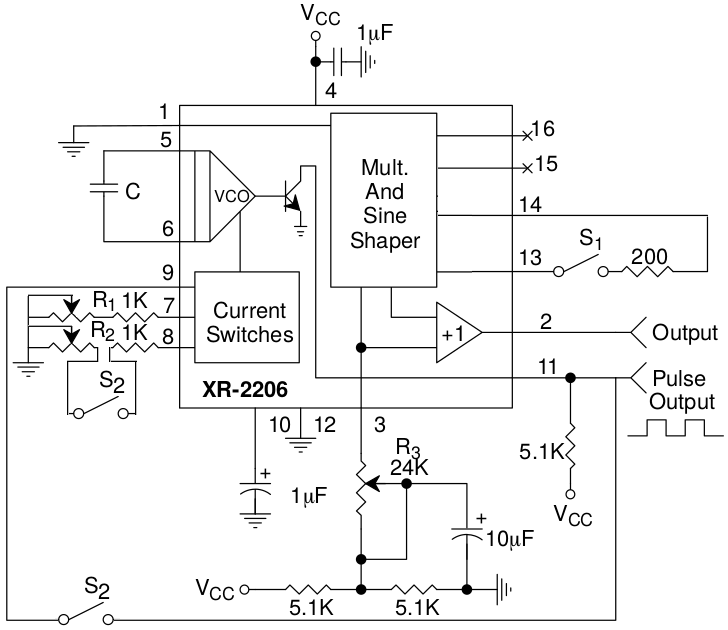
\includegraphics[width=9.5cm]{modulator}
    \caption{Esquemático del modulador.}
    \label{fig:schematicModulator} 
  \end{subfigure}

  \begin{subfigure}[b]{0.65\textwidth}
    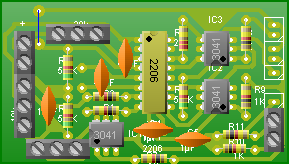
\includegraphics[width=9.5cm]{pcbModulator}
    \caption{PCB del modulador.}
    \label{fig:pcbModulator}
  \end{subfigure}

  \begin{subfigure}[b]{0.65\textwidth}
    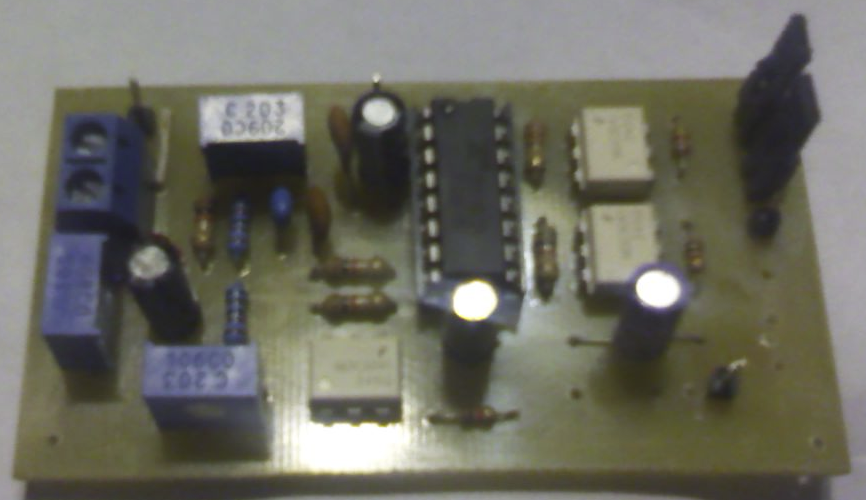
\includegraphics[width=9.5cm]{realModulator}
    \caption{Circuito construido del modulador.}
  \end{subfigure}
  \caption{Distintas etapas en la construcción del Modulador del radar.}
\end{figure}


\subsection{Electrónica de RF}

Se decidió utilizar como base la electrónica RF de un radar FMCW de banda S de baja potencia diseñado por el Instituto de Tecnología de Massachusetts (MIT). La cual posee una potencia de transmisión igual a $\SI{12}{\dBm}$. Con esto se define el requerimiento \ref{req:l2_txPower}.

La cadena está compuesta por un generador controlado por tensión (VCO), atenuadores, divisores de potencia, amplificadores y un mezclador, ver figura \ref{fig:rfElectronics}. A continuación se describen las principales características de cada uno de los componentes mencionados.

\begin{figure}[htb]
  \centering
  \begin{subfigure}{\textwidth}
    \centering
    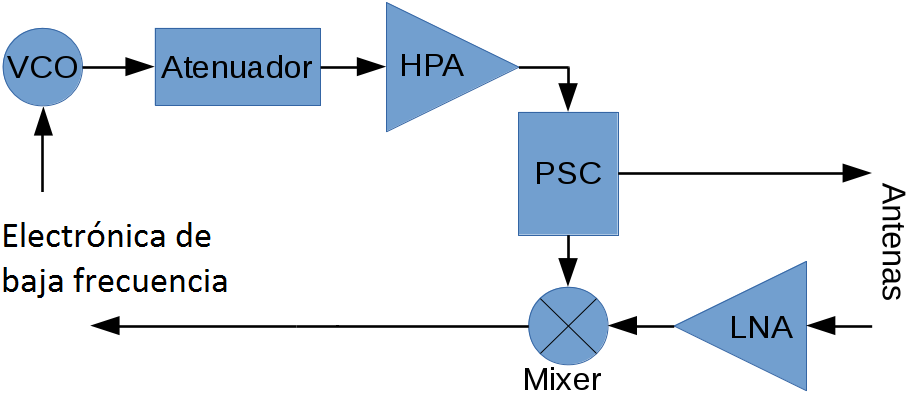
\includegraphics[width=10cm]{rfElectronics}
    \caption{Circuito esquemático}
  \end{subfigure}

  \begin{subfigure}{\textwidth}
    \centering
    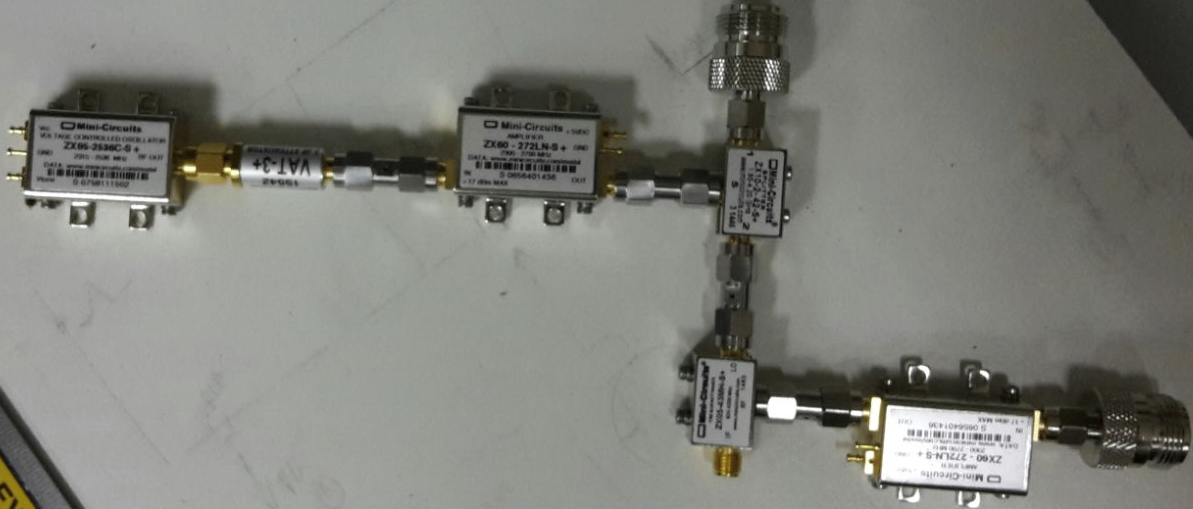
\includegraphics[width=10cm]{rfElectronics2}
    \caption{Electrónica de RF armada.}
  \end{subfigure}
  \caption{Distintas etapas en la construcción de la electrónica de RF.}
  \label{fig:rfElectronics}
\end{figure}

\begin{description}
  \item[VCO] El código de dicho componente es ZX95-2536C \cite{VCOMiniCircuits}. La frecuencia de la señal transmitida depende de la tensión de entrada, dicha dependencia puede observarse en la figura \ref{fig:freqVsVoltage}. La potencia transmitida es de $\SI{6.2}{\dBm}$ cuando la tensión de alimentación es de $\SI{5}{V}$. La frecuencia central de trabajo es igual a $\SI{2450}{\MHz}$ y posee un ancho de banda de transmisión máximo igual a $\SI{300}{\MHz}$. De esta forma se definen los requerimientos \ref{req:l2_f0} y \ref{req:l2_bw}.
  \begin{figure}[H]
   \centering
   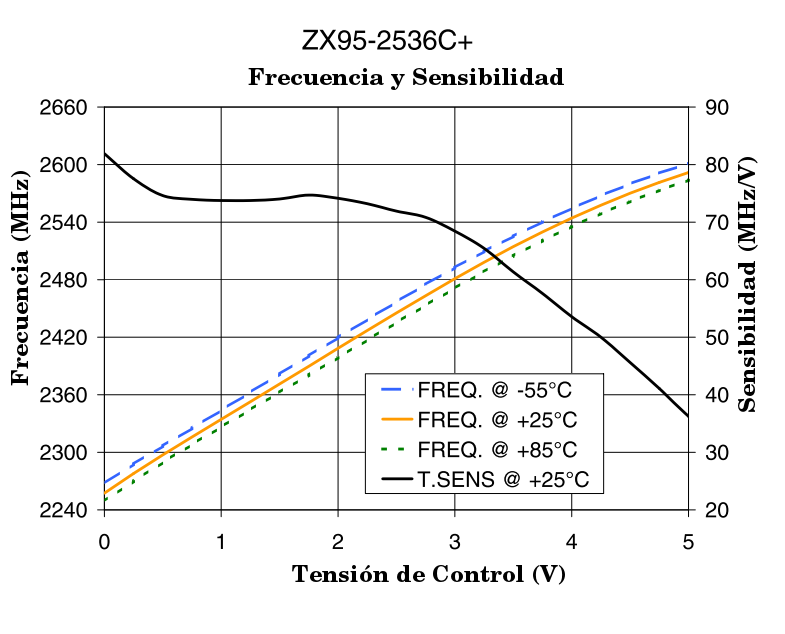
\includegraphics[width=10cm]{frequencyVsVoltage}
   \caption{Frecuencia generada en función de la tensión de control \cite{VCOMiniCircuits}.}
   \label{fig:freqVsVoltage}
  \end{figure}
  
  \item[Atenuador] El código de dicho componente es VAT-3 \cite{AttMiniCircuits}. En la frecuencia de trabajo del VCO, la señal es atenuada en $\SI{3.2}{\deci\bel}$. El mismo es utilizado para proteger al generador ante cualquier señal reflejada por desadaptaciones o por mal conexionado del instrumental.

  \item[Divisor de potencia] El código de dicho componente es ZX10-2-42 \cite{PSCMiniCircuits}. El mismo posee una pérdida por inserción desde el puerto central a los individuales igual a $\SI{3.26}{\dB}$ en una frecuencia de $\SI{2460}{\MHz}$. La figura \ref{fig:insertionLoss} muestra dicha pérdida en función de la frecuencia de trabajo.

  \begin{figure}[H]
   \centering
   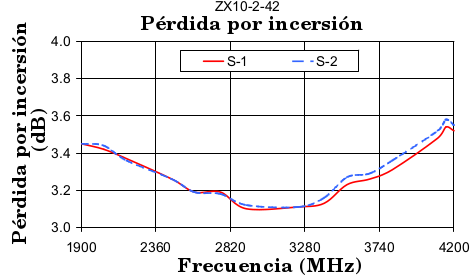
\includegraphics[width=10cm]{insertionLoss}
   \caption{Pérdida de inserción en el divisor de potencia \cite{PSCMiniCircuits}.}
   \label{fig:insertionLoss}
  \end{figure}

  \item[Amplificador] El código de dicho componente es ZX60-272LN \cite{LNAMiniCircuits}. Según la hoja de datos, el mismo posee una ganancia igual a $\SI{14}{\deci\bel}$ para la frecuencia central de trabajo del VCO.

  \item[Mezclador] El código de dicho componente es ZX05-43MH \cite{mixerMiniCircuits}. Según la hoja de datos, el mismo posee una pérdida por conversión igual a $\SI{5.5}{\deci\bel}$ para la frecuencia central de trabajo del VCO.

\end{description}


\subsection{Antenas}

Las antenas escogidas son del tipo apertura dado que se requiere cierta direccionalidad. A su vez, se decide utilizar una para transmitir y otra para recibir. Por cada cavidad hay dos monopolos distribuidos de forma ortogonal entre sí para poder transmitir y recibir en ambas polarizaciones, horizontal (H) y vertical (V). De esta forma se definen los requerimientos \ref{req:l2_antQuantity}, \ref{req:l2_antenna} y \ref{req:l2_polarization}. Los atributos a definir son la altura de la pesca, la distancia de la misma a la pared de la cavidad, la longitud y diámetro del caño. Los mismos dependen de la frecuencia de trabajo y el modo en que se desee trabajar.

\begin{figure}
 \centering
 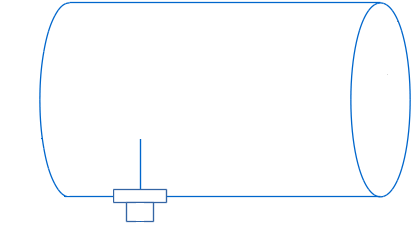
\includegraphics[width=8cm]{antennas}
 \caption{Dimensiones de una guía de onda de medio caño.}
 \label{fig:antennas}
\end{figure}

Cada modo de resonancia es definido por una frecuencia de corte inferior, el cual no podría existir a frecuencias inferiores. El modo dominante es el que posee la menor frecuencia de corte posible. Para este tipo de guías de ondas es el TE$_{11}$. En este modo no hay campo eléctrico en la dirección de la propagación de la onda y define la relación entre el radio de la antena, $R$, y la frecuencia de corte \cite{circularWaveguides}.
\begin{equation} \label{eq:freqInf}
  f_c = \dfrac{\num{1.8412}}{2\pi R} c
\end{equation}

La longitud de onda dentro de la guía es mayor a la de la señal en espacio libre y responde a la siguiente ecuación,
\begin{equation} \label{eq:lambdaInGuide}
\lambda_g = \begin{cases} \dfrac{\lambda}{\sqrt{1 - (\dfrac{f_c}{f})^2}}, & \mbox{donde } f > f_c \\ \infty, & \mbox{donde } f = f_c \end{cases}
\end{equation}

Se debe elegir el tamaño de la guía de forma tal que el ancho de banda de operación entre completamente dentro de dicho modo de de resonancia, por lo tanto la máxima frecuencia de trabajo debe ser menor a la frecuencia de corte de TE$_{21}$ \cite{circularWaveguides},
\begin{equation} \label{eq:freqSup}
  f_{csup} = \dfrac{\num{3.0542}c}{2\pi R}
\end{equation}

\begin{description}
  \item[Altura de la pesca] Este atributo se corresponde con el requerimiento \ref{req:l2_pescaLength} y se define como la cuarta parte de la longitud de onda de la señal transmitida en espacio libre. En este caso se utiliza la frecuencia central de trabajo.

  \begin{equation}
  WireLength = \dfrac{\lambda}{4}
  \end{equation}

Dado que la frecuencia de trabajo utilizada es igual a $\SI{2450}{\MHz}$, la longitud de la pesca resulta aproximadamente igual a $\SI{3}{\centi\meter}$.

  \item[Longitud y diámetro de la guía de onda circular] Estos atributos se corresponden con el requerimiento \ref{req:l2_cavity}. Como se mencionó previamente, las frecuencias de cortes inferiores de cada modo de resonancia depende del diámetro de la guía de ondas, por lo tanto el ancho de banda de cada modo se encuentra determinado por las mismas. Y como se desea que las frecuencias de trabajo, $\SI{2300}{\MHz} - \SI{2600}{\MHz}$, entren dentro del modo dominante, el diámetro máximo y mínimo admisible es de,
  \begin{equation}
  \SI{7.64}{\centi\meter} < D < \SI{11.2}{\centi\meter}
  \end{equation}

  El resultado anterior fue obtenido siguiendo las ecuaciones \ref{eq:freqInf} y \ref{eq:freqSup}. La antena que se consiguió posee una longitud igual a $\SI{15}{\centi\meter}$ y un diámetro igual a $\SI{10}{\centi\meter}$, por lo tanto, el ancho de banda admisible del modo dominante es de $\SI{1157.5}{\MHz}$ con una frecuencia central de $\SI{2335.75}{\MHz}$.

  \item[Distancia monopolo a la pared de la guía de onda] Este atributo se corresponde con el requerimiento \ref{req:l2_cavityDistance}. Dado que la guía de onda es cilíndrica y que el monopolo transmite omnidireccionalmente en el plano perpendicular al mismo \cite{arrl2007}, parte de la onda se transmite hacia el frente de la guía pero otra parte hacia el fondo, la misma se refleja con la pared metálica volviendo al punto de origen con dirección del frente de la antena.

  Para que la interferencia de ondas sea constructiva, es necesario que el eco posea la misma fase que la señal a transmitir. Se logra el efecto deseado si la separación entre el monopolo y la pared es de $\frac{\lambda}{4}$, dado que el eco en un medio metálico implica un desfase de $\SI{180}{\degree}$. Siguiendo la ecuación \ref{eq:lambdaInGuide}, y dado que la frecuencia central de trabajo es de $\SI{2450}{\MHz}$, la longitud de onda dentro de la guía de onda es igual a $\SI{17.56}{\centi\meter}$, por lo tanto la distancia resultante es $\SI{4.39}{\centi\meter}$.

\end{description}

\subsection{Pasa Bajos}

El circuito pasa bajos del receptor, utilizado para filtrar todas las frecuencias salvo las pertenecientes al rango de trabajo del radar, es el sallen-key \cite{Unwin2003}. Este circuito, ilustrado en la figura \ref{fig:lowPassCircuit}, consta de tres etapas. La primera es un amplificador no inversor y las siguientes son pasa bajos de segundo orden con una frecuencia de corte del orden de $\SI{20}{\kHz}$, conformando un circuito de cuarto orden con una frecuencia de corte igual a los $\SI{20}{\kHz}$, definiéndose así el requerimiento \ref{req:l2_filter}. Dicho valor surge de que la señal, luego de ser filtrada, se recibe en la computadora a través del jack del micrófono, el cual posee una frecuencia de muestreo de $\SI{40}{\kHz}$. Por lo tanto, para cumplir con el teorema de nyquist, si se desea evitar el aliasing en la señal, la frecuencia máxima no puede superar $\SI{20}{\kHz}$.

Cabe destacar que, como el radar trabaja con tensiones de $\SI{12}{\volt}$ y $\SI{5}{\volt}$, los amplificadores están alimentados con la tensión de mayor denominación y las resistencias conectadas a sus pines inversores con la tensión de menor denominación.

\begin{figure}
 \centering
 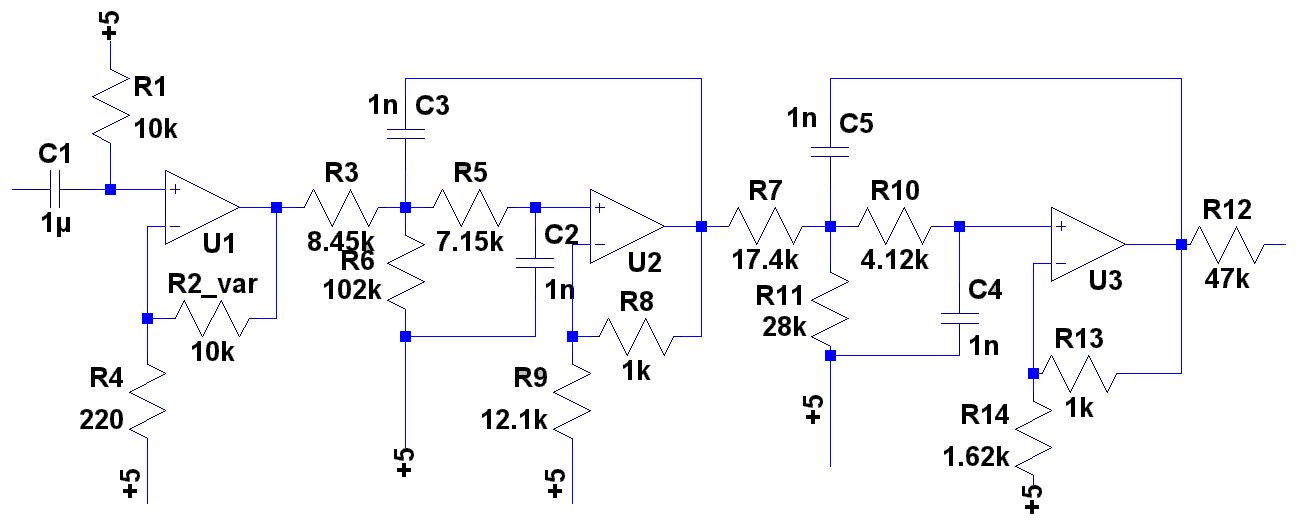
\includegraphics[width=15cm]{lowPassBand}
 \caption{Circuito pasa bajos y amplificador de señal.}
 \label{fig:lowPassCircuit}
\end{figure}

La entrada al circuito amplificador posee un capacitor en serie para eliminar el offset de la señal de entrada y una resistencia conectada a los $\SI{5}{\volt}$ estableciendo el offset común. La existencia del capacitor en serie a la señal resulta en un circuito pasa altos, con una frecuencia de corte inferior igual a
\begin{equation}\label{eq:fcInf}
  fc = \dfrac{1}{2\pi R_1 C_1} = \SI{7.23}{\Hz}
\end{equation}

La ecuación \ref{eq:gainAmplifier} es la transferencia de este circuito para cuando se considera despreciable la influencia del capacitor serie sobre la señal.
\begin{equation}\label{eq:gainAmplifier}
  Av = 1 + \dfrac{R_2}{R_4}
\end{equation}

Las siguientes etapas fueron caracterizadas utilizando las ecuaciones que definen al filtro sallen-key, listadas en la referencia \cite{Unwin2003}. Pero, como dichos circuitos no son exactamente iguales por la existencia de las resistencias $R_6$ y $R_{11}$ de la figura \ref{fig:lowPassCircuit}, dichas ecuaciones no pueden ser utilizadas directamente. Si se realiza un corte en cada etapa, como se muestra en la figura \ref{fig:genericSallen}, para calcular el equivalente de thevenin, se obtiene el circuito mostrado en la figura \ref{fig:genericSallen2}.

\begin{figure}
  \centering
  \begin{subfigure}{0.4\textwidth}
    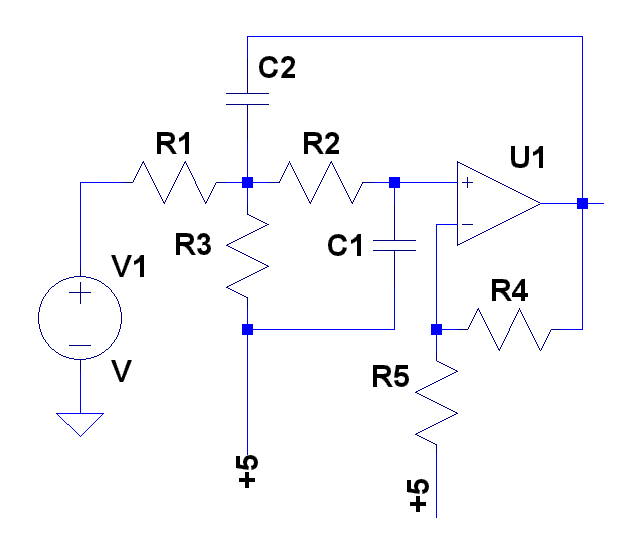
\includegraphics[width=6cm]{genericSallenKey}
    \caption{Etapa generica del circuito pasa bajo del radar}
    \label{fig:genericSallen}   
  \end{subfigure}
  {\color{blue}\LARGE$\Rightarrow$}
  \begin{subfigure}{0.4\textwidth}
    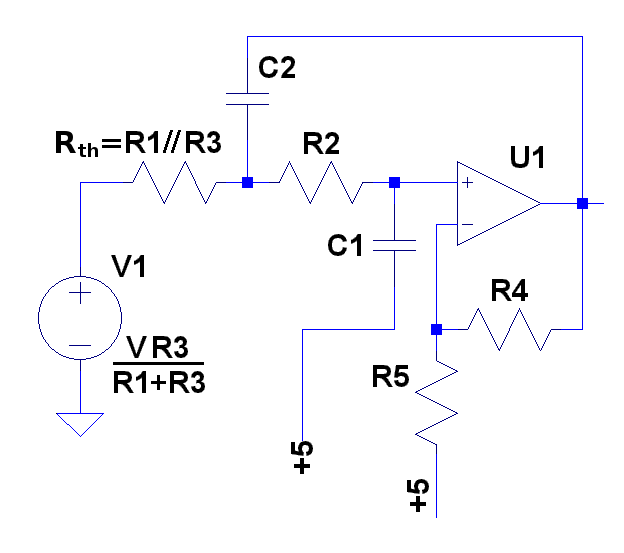
\includegraphics[width=6cm]{genericSallenKey2}
    \caption{Equivalente del circuito pasa bajos del radar}
    \label{fig:genericSallen2}
  \end{subfigure}             
  \caption{Equivalente filtro Sallen-key}
\end{figure}
Manteniendo la nomenclatura de los componentes mostrados en la figura \ref{fig:genericSallen2}, las ecuaciones para calcular la ganancia a bajas frecuencias, la frecuencia de corte y el Q de cada etapa son \ref{eq:gainLowPass}, \ref{eq:f0LowPass} y \ref{eq:qLowPass} respectivamente.
\begin{equation}\label{eq:gainLowPass}
  Av = 1 + \dfrac{R_4}{R_5}
\end{equation}
\begin{equation}\label{eq:f0LowPass}
  f_0 = \dfrac{1}{2\pi\sqrt{R_{th}R_2C_1C_2}}
\end{equation}
\begin{equation}\label{eq:qLowPass}
  Q = \dfrac{\sqrt{R_{th}R_2C_1C_2}}{R_{th}C_1 + R_2C_1 + \dfrac{R_{th}C_2R_4}{R_5}}
\end{equation}

La tabla \ref{tab:lowPassProperties} resume la ganancia y frecuencias de corte y Q de cada etapa.

\begin{table}[htb]
  \caption{Propiedades de las etapas del filtro del receptor.}
  \centering
  \label{tab:lowPassProperties}
  \begin{tabular}{l c c c}
  \toprule
  \textbf{Etapa} & \textbf{Ganancia} & \textbf{Frecuencia Corte} & \textbf{Q} \tabularnewline
   & [veces] & [Hz] & \tabularnewline
  \midrule
  Primera & 1 - 46,45 & - & - \tabularnewline

  segunda & 1,08 & 21306 & 0,52 \tabularnewline

  tercera & 1,62 & 23935 & 0,8 \tabularnewline

  \bottomrule
  \end{tabular}
\end{table}

Las imágenes de la figura \ref{fig:lowPassFilterCircuit} muestran el PCB y el circuito pasa bajos armado.
\begin{figure}[H]
  \centering
  \begin{subfigure}[b]{0.47\textwidth}
    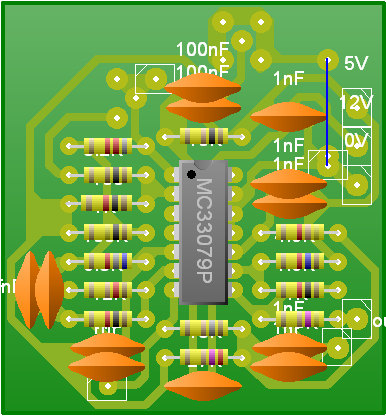
\includegraphics[width=7cm]{pcbLPF}
    \caption{PCB del filtro pasa bajos.}
  \end{subfigure}
  \begin{subfigure}[b]{0.47\textwidth}
    \includegraphics[width=7cm]{lowPassFilter}
    \caption{Circuito construido del filtro pasa bajos.}
  \end{subfigure}
  \caption{Distintas etapas en la construcción del filtro pasa bajos del radar.}
  \label{fig:lowPassFilterCircuit}
\end{figure}


\subsection{Procesador}

Dado que el procesador es software, se lo detallará junto al simulador en el capítulo \ref{ch:softwareDevelopment}.

\subsection{Gabinete}

El hecho de querer montar en un futuro al radar en un dron introduce ciertos requerimientos de volumen y peso que afectan en la decisión del gabinete a utilizar, como el que no debe pesar más de $\SI{1}{\kg}$. Dado que se requiere que sea lo más liviano posible y en un volumen determinado, se optó por utilizar plástico como material. El compuesto del mismo es poliestireno de alto impacto y es fabricado con la técnica de termoformado. El peso final del radar resulta ser de $\SI{600}{\gram}$ cumpliéndose el requerimiento \ref{req:l2_weight}.

Como habrán otros componentes electrónicos que pueden afectar al funcionamiento del radar por interferencia electromagnéticas (EMI), se debe metalizar el gabinete. Una de las posibles estrategias es la del metalizado al vacío, aunque dicho proceso quedará como trabajo futuro.

La figura \ref{fig:radar3D} muestran la modelización del radar completo, como se vería el interior como el exterior del mismo.
\begin{figure}[H]
 \centering
 \begin{subfigure}[t]{0.49\textwidth}
    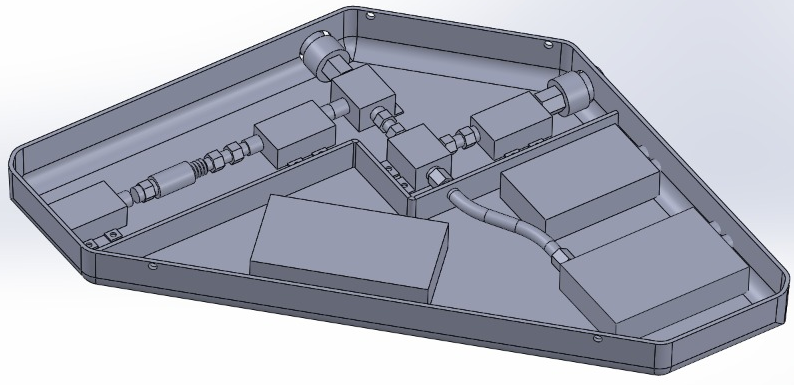
\includegraphics[width=7.5cm]{radar3D}
  \end{subfigure}
  \begin{subfigure}[t]{0.49\textwidth}
    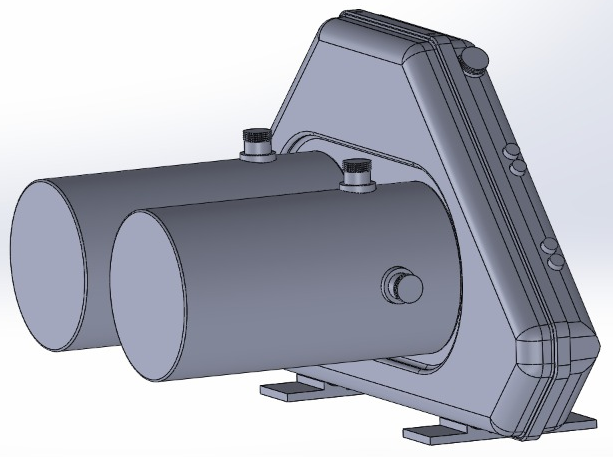
\includegraphics[width=7.5cm]{completeRadar}
  \end{subfigure}
 \caption{Modelo del gabinete interna y exterma.}
 \label{fig:radar3D}
\end{figure}

La figura \ref{fig:completeRadar} muestra tanto el interior del gabinete armado con la distribución de los componentes dentro del mismo como el radar de perfil.

\begin{figure}[H]
 \centering
 \begin{subfigure}[t]{0.8\textwidth}
    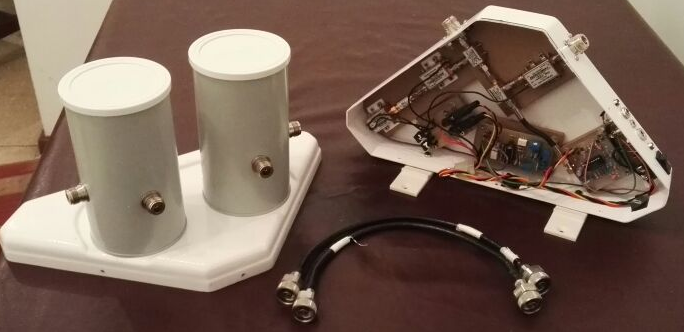
\includegraphics[width=12cm]{openedRuiltRadar}
  \end{subfigure}

  \begin{subfigure}[t]{0.5\textwidth}
    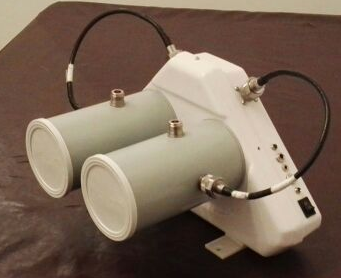
\includegraphics[width=7.5cm]{completeBuiltRadar}
  \end{subfigure}
 \caption{Modelo del gabinete interna y exterma.}
 \label{fig:completeRadar}
\end{figure}


\section{Mediciones de funcionamiento}

En esta sección se muestran distintas mediciones sobre diversos módulos del radar para caracterizarlo.
Los instrumentos utilizados son
\begin{itemize}
  \item Analizador de espectros: Rhode \& Schwartz ESU 40 \cite{spectrumAnalyzer}.
  \item Analizador de redes Vectorial (VNA): Keysight Technologies N9923A FieldFox RF.
Vector Network Analyzer \cite{VNA}.
  \item Osciloscopio: Goodwill, GOS-653G
  \item Contador: GoodWill, GUC-2020
  \item Generador de señales: Topward, FG-8140
\end{itemize}

\subsection{Transferencia, filtro pasa bajos}

Para la medición de la función de transferencia del filtro se utilizó un generador de señales, un osciloscopio y un contador. Al primero se lo conectó a la entrada del circuito. Al resto del instrumental se lo conectó tanto a la entrada como a la salida del mismo. La figura \ref{fig:lowPassFilterConnections} muestra el banco de trabajo utilizado para realizar la medición.

\begin{figure}[H]
 \centering
 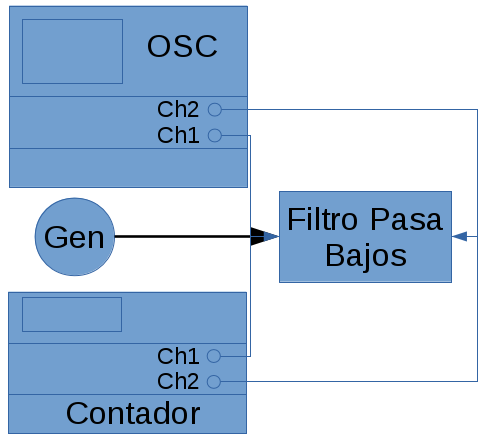
\includegraphics[width=6cm]{lowPassFilterTransferenceWorkbench}
 \caption{Banco de medición, transferencia del filtro pasa bajos.}
 \label{fig:lowPassFilterConnections}
\end{figure}

Durante el ensayo se midió tanto la tensión de entrada como la de salida con el osciloscopio a medida que se fue variando la frecuencia del generador para determinar la ganancia del circuito. A su vez, con el contador se determinó el desfase entre ambas señales midiendo el intervalo de tiempo entre los flancos ascendentes de cada una. La tabla \ref{tab:lowPassFilterTransference} y la figura \ref{fig:lowPassFilterTransference} muestran los resultados obtenidos.

La incertidumbre de las mediciones de tensiones medidas es del $\SI{3}{\percent}$. Por lo tanto la incertidumbre de la ganancia es del $\SI{6}{\percent}$. En cambio, la incertidumbre del intervalo de tiempo y el de la frecuencia ronda el $\SI{1}{\percent}$ dado que el instrumento fue configurado para disminuir la incertidumbre asociada a la medición. Por lo tanto la incertidumbre del desfase es del $\SI{2}{\percent}$. La tabla \ref{tab:lowPassFilterTransference} y la figura \ref{fig:lowPassFilterTransference} muestran los resultados obtenidos.

En la figura \ref{fig:lowPassFilterTransference} se muestran dos curvas, en rojo la ganancia y en azul la fase en función de la frecuencia. Se puede observar que el ancho de banda del circuito es aproximadamente de $\SI{20}{\kHz}$ con una frecuencia de corte inferior igual a $\SI{10}{\Hz}$. Es importante notar que la misma es plana hasta una frecuencia de $\SI{10}{\kHz}$. En cambio, observando el desfase del circuito, el mismo es igual a $\SI{0}{\degree}$ en un rango de frecuencias de $\SI{30}{\Hz}$ a $\SI{2}{\kHz}$. Si la señal recibida se encuentra en otros valores de frecuencias, habría que substraer el efecto de este subsistema sobre la misma para eliminar el error sistemático. De esta forma se verifica el requerimiento \ref{req:l2_filter}.

\begin{table}[H]
  \caption{Transferencia del circuito pasa bajos.}
  \centering
  \label{tab:lowPassFilterTransference}
  \begin{tabular}{S[table-auto-round, table-format=5.2] *{2}{S[table-auto-round, table-format=1.2]} S[table-auto-round, table-format=-4.2] S[table-auto-round, table-format=2.1] S[table-auto-round, table-format=-3]}
  \toprule
  
  {\textbf{Frec}} & \textbf{Vin} & \textbf{Vout} & \textbf{Intervalo de T} & \textbf{Ganancia} & \textbf{Desfase} \tabularnewline
  
   {[$\si{\Hz}$]} & {[$\si{\V}$]} & {[$\si{\V}$]} & {[$\si{\mu\sec}$]} & {[$\si{\dB}$]} & {[$\si{\degree}$]} \tabularnewline
  
  \midrule
  9.97 & 0.6 & 1.48 & -7462 & 7.8422093002 & 26.7826104 \tabularnewline

  20 & 0.6 & 1.95 & -905 & 10.2376672196 & 6.516 \tabularnewline

  29.37 & 0.6 & 2 & 0 & 10.4575749056 & 0 \tabularnewline

  51.11 & 0.6 & 2 & 0 & 10.4575749056 & 0 \tabularnewline

  100 & 0.6 & 2.1 & 0 & 10.881360887 & 0 \tabularnewline

  192 & 0.6 & 2.1 & 0 & 10.881360887 & 0 \tabularnewline

  305 & 0.6 & 2 & 0 & 10.4575749056 & 0 \tabularnewline

  400 & 0.6 & 2 & 13.37 & 10.4575749056 & -1.92528 \tabularnewline

  500 & 0.6 & 2 & 15.99 & 10.4575749056 & -2.8782 \tabularnewline

  600 & 0.6 & 2 & 16.45 & 10.4575749056 & -3.5532 \tabularnewline

  700 & 0.6 & 2 & 17.86 & 10.4575749056 & -4.50072 \tabularnewline

  800 & 0.6 & 2 & 18.65 & 10.4575749056 & -5.3712 \tabularnewline

  900 & 0.6 & 2 & 19.28 & 10.4575749056 & -6.24672 \tabularnewline

  1000 & 0.6 & 2 & 19.75 & 10.4575749056 & -7.11 \tabularnewline

  2000 & 0.6 & 2 & 12.48 & 10.4575749056 & -8.9856 \tabularnewline

  3000 & 0.6 & 2 & 15.8 & 10.4575749056 & -17.064 \tabularnewline

  4000 & 0.6 & 2 & 17.77 & 10.4575749056 & -25.5888 \tabularnewline

  5050 & 0.6 & 2 & 18.95 & 10.4575749056 & -34.4511 \tabularnewline

  6000 & 0.6 & 2 & 19.66 & 10.4575749056 & -42.4656 \tabularnewline

  7000 & 0.6 & 2 & 20.14 & 10.4575749056 & -50.7528 \tabularnewline

  8000 & 0.6 & 2 & 20.64 & 10.4575749056 & -59.4432 \tabularnewline

  9000 & 0.6 & 2 & 21.01 & 10.4575749056 & -68.0724 \tabularnewline

  10020 & 0.6 & 2 & 21.34 & 10.4575749056 & -76.977648 \tabularnewline

  11000 & 0.6 & 2 & 21.63 & 10.4575749056 & -85.6548 \tabularnewline

  12000 & 0.6 & 1.85 & 21.98 & 9.7804095604 & -94.9536 \tabularnewline

  13000 & 0.6 & 1.85 & 22.27 & 9.7804095604 & -104.2236 \tabularnewline

  14000 & 0.6 & 1.8 & 22.56 & 9.5424250944 & -113.7024 \tabularnewline

  15000 & 0.6 & 1.8 & 22.7 & 9.5424250944 & -122.58 \tabularnewline

  16000 & 0.6 & 1.75 & 22.92 & 9.2977359661 & -132.0192 \tabularnewline

  17000 & 0.6 & 1.7 & 23.07 & 9.0459534199 & -141.1884 \tabularnewline

  18000 & 0.6 & 1.6 & 23.29 & 8.5193746454 & -150.9192 \tabularnewline

  20000 & 0.6 & 1.44 & 23.72 & 7.6042248342 & -170.784 \tabularnewline

  26000 & 0.62 & 1 & 24.52 & 4.15216621 & -229.5072 \tabularnewline
  \bottomrule
  \end{tabular}
\end{table}

\begin{figure}[H]
 \centering
 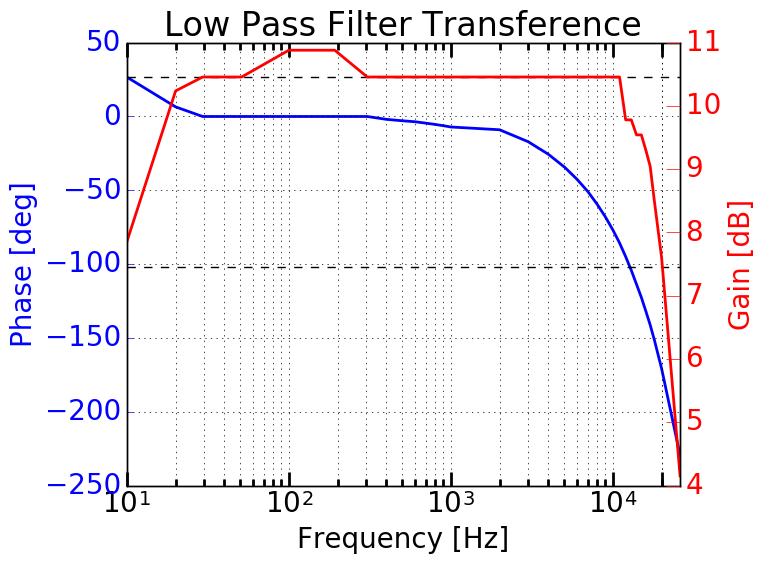
\includegraphics[width=12cm]{transference}
 \caption{Transferencia del circuito pasa bajos. En rojo la ganancia y en azul el desfase.}
 \label{fig:lowPassFilterTransference}
\end{figure}


\subsection{Potencia transmitida}

Para la medición de la potencia transmitida del radar se utilizó el analizador de espectros conectado en el cable que une la antena transmisora con el resto de la electrónica del radar. La figura \ref{fig:txPowerConnections} muestra el banco de trabajo utilizado para realizar la medición.

\begin{figure}[H]
 \centering
 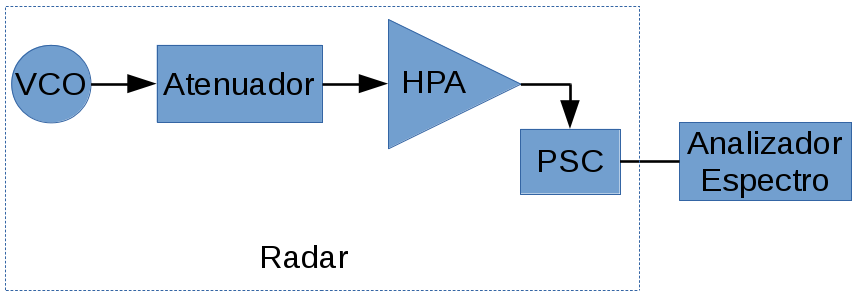
\includegraphics[width=10cm]{txPowerWorkbench}
 \caption{Banco de medición, potencia transmitida del radar.}
 \label{fig:txPowerConnections}
\end{figure}

La tabla \ref{tab:PNAConfigTxPower} resume las configuraciones utilizadas en el analizador de espectros para la medición y la figura \ref{fig:txPowerMeasurements} muestra el resultado de la medición.

\begin{table}[H]
  \caption{Configuración del analizador de espectros para medir la potencia transmitida del radar.}
  \centering
  \label{tab:PNAConfigTxPower}
  \begin{tabular}{l c c}
  \toprule
  \textbf{Característica} & \textbf{Configuración} & \textbf{Unidad} \tabularnewline
  \midrule
  Mode & ANALYZER & \tabularnewline

  Center Freq & 2434262820,514000 & \si{\hertz} \tabularnewline

  Freq Offset & 0,000000 & \si{\hertz} \tabularnewline

  Span & 1000000000,000000 & \si{\hertz} \tabularnewline

  x-Axis & LIN & \tabularnewline

  Start & 1934262820,514000 & \si{\hertz} \tabularnewline

  Stop & 2934262820,514000 & \si{\hertz} \tabularnewline

  Ref Level & 18,000000 & \si{\dBm} \tabularnewline

  Level Offset & 0,000000 & \si{\deci\bel} \tabularnewline

  Ref Position & 100,000000 & \si{\percent} \tabularnewline

  y-Axis & LOG & \tabularnewline

  Level Range & 50,000000 & \si{\deci\bel} \tabularnewline

  Rf Att & 70,000000 & \si{\deci\bel} \tabularnewline

  RBW & 10000000,000000 & \si{\hertz} \tabularnewline

  VBW & 10000000,000000 & \si{\hertz} \tabularnewline

  SWT & 0,002500 & \si{\second} \tabularnewline

  Trace Mode & CLR/WRITE & \tabularnewline

  Detector & RMS & \tabularnewline

  Sweep Count & 0 & \tabularnewline

  \bottomrule
  \end{tabular}
\end{table}

En la figura \ref{fig:txPowerMeasurements} se puede observar que la potencia transmitida por el radar es de $\SI{11.87}{\dBm}$ en una frecuencia central igual a $\SI{2.43}{\giga\hertz}$ y que el piso de ruido para esta medición se encuentra entre los $\SI{-14}{\dBm}$ y $\SI{-17.4}{\dBm}$. De esta forma se valida el requerimiento \ref{req:l2_txPower}.

\begin{figure}[H]
 \centering
 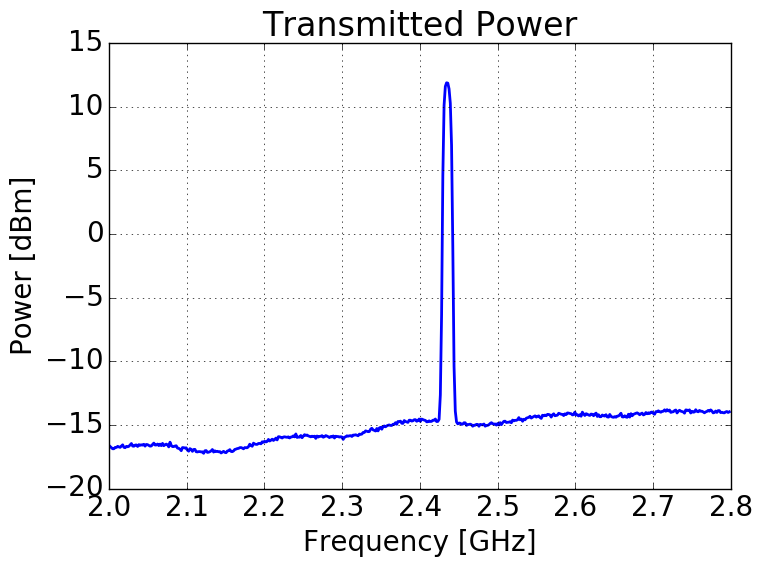
\includegraphics[width=9cm]{txPower}
 \caption{Potencia transmitida del radar medida con un PNA.}
 \label{fig:txPowerMeasurements}
\end{figure}


\subsection{Ancho de banda}

Para la medición del ancho de banda transmitido se utiliza el analizador de espectros conectado en el cable que une la antena transmisora con el resto de la electrónica del radar. La figura \ref{fig:bartPowerConnections} muestra el banco de trabajo utilizado para realizar la medición.

\begin{figure}[H]
 \centering
 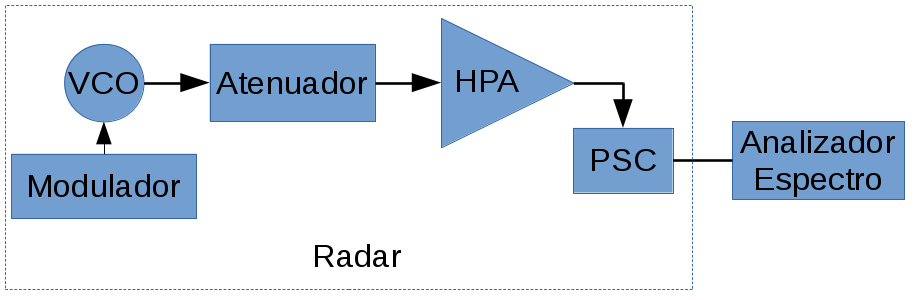
\includegraphics[width=10cm]{bartPowerWorkbench}
 \caption{Banco de medición, cabeza de chirp transmitida del radar.}
 \label{fig:bartPowerConnections}
\end{figure}

La tabla \ref{tab:PNAConfigBartPower} resume las configuraciones utilizadas en el analizador de espectros para la medición y la figura \ref{fig:bartPowerMeasurements} muestra el resultado de la medición.

\begin{table}[H]
  \caption{Configuración del analizador de espectros, medición del BW transmitido del radar.}
  \centering
  \label{tab:PNAConfigBartPower}
  \begin{tabular}{l c c}
  \toprule
  \textbf{Característica} & \textbf{Configuración} & \textbf{Unidad} \tabularnewline
  \midrule
  Mode & ANALYZER & \tabularnewline

  Center Freq & 2450288461,540000 & \si{\hertz} \tabularnewline

  Freq Offset & 0,000000 & \si{\hertz} \tabularnewline

  Span & 1000000000,000000 & \si{\hertz} \tabularnewline

  x-Axis & LIN & \tabularnewline

  Start & 1950288461,540000 & \si{\hertz} \tabularnewline

  Stop & 2950288461,540000 & \si{\hertz} \tabularnewline

  Ref Level & 18,000000 & \si{\dBm} \tabularnewline

  Level Offset & 0,000000 & \si{\deci\bel} \tabularnewline

  Ref Position & 100,000000 & \si{\percent} \tabularnewline

  y-Axis & LOG & \tabularnewline

  Level Range & 50,000000 & \si{\deci\bel} \tabularnewline

  Rf Att & 70,000000 & \si{\deci\bel} \tabularnewline

  RBW & 10000000,000000 & \si{\hertz} \tabularnewline

  VBW & 10000000,000000 & \si{\hertz} \tabularnewline

  SWT & 0,002500 & \si{\second} \tabularnewline

  Trace Mode & MAXHOLD & \tabularnewline

  Detector & RMS & \tabularnewline

  Sweep Count & 0 & \tabularnewline
  \bottomrule
  \end{tabular}
\end{table}

\begin{figure}[H]
 \centering
 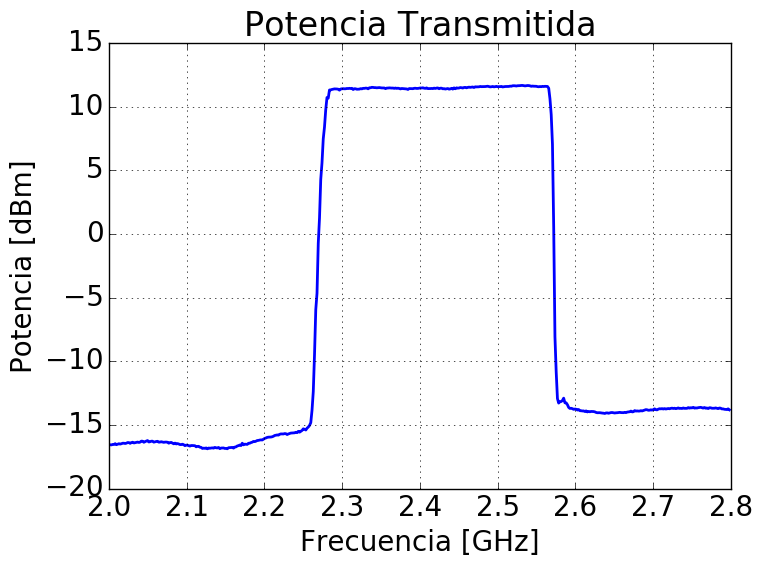
\includegraphics[width=10cm]{chripHeadPower}
 \caption{Potencia transmitida del radar medida con un analizador de espectros.}
 \label{fig:bartPowerMeasurements}
\end{figure}

Se puede observar que el ancho de banda de la señal transmitida, a $\SI{-3}{\dB}$ con respecto al pico, es igual a $\SI{291.67}{\mega\hertz}$. A su vez, la potencia de la señal es de $\SI{12}{\dBm}$ mientras que el piso de ruido es de $\SI{-15}{\dBm} \pm \SI{2}{\dBm}$. De esta forma se verifica el requerimiento \ref{req:l2_bw}.


\subsection{Parámetros S de las antenas} \label{ssc:sParameters}

Esta medición está diseñada para caracterizar el comportamiento de las antenas tanto de forma individual, midiendo el coeficiente de reflexión $S_{11}$ de cada una, como de forma grupal, midiendo el coeficiente de transmisión $S_{21}$ entre las mismas. Idealmente estos valores deberían ser 0, dado que mientras más alejado a dicho valor sea el $S_{11}$, menor es la potencia que ingresa a la antena. En cambio, el parámetro $S_{21}$ está relacionado directamente con el acoplamiento mutuo entre las antenas. Mientras mayor es dicho valor, mayor potencia recibe la antena receptora, lo cual es un efecto indeseado dado que ya se estaría recibiendo señal sin siquiera haber presencia de un blanco iluminado a caracterizar.

El banco de medición está compuesto por un VNA en donde cada canal del mismo está conectado a una antena del radar, de esta forma  la señal se transmite por una antena y se recibe a través de la segunda, ver figura \ref{fig:sParamsConnections}.
\begin{figure}[H]
 \centering
 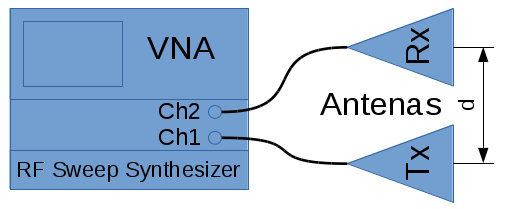
\includegraphics[width=8cm]{sParamsAntenaWorkbench}
 \caption{Banco de medición, parámetros S de las antenas.}
 \label{fig:sParamsConnections}
\end{figure}

Como las antenas son plarimétricas, se repitió la medición en todas las posibles combinaciones de polarizaciones, HH, HV, VH y VV. Es importante notar que la distancia entre los centros de las antenas permaneció invariante e igual a $\SI{15.5}{\centi\meter}$. La figura \ref{fig:sParametersMeasurements} posee los resultados de los cuatro ensayos.

\begin{figure}[H]
  \centering
  \begin{subfigure}{0.47\textwidth}
    \centering
    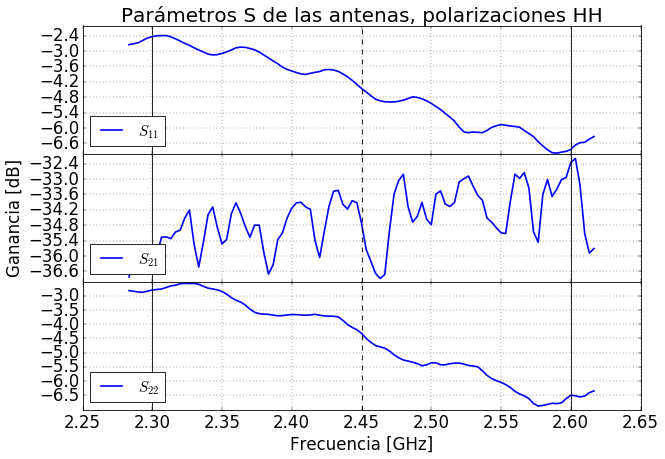
\includegraphics[width=7cm]{SParamsHH}
    \caption{Polarización HH}
    \label{subfig:hhPol}
  \end{subfigure}
  \begin{subfigure}{0.47\textwidth}
    \centering
    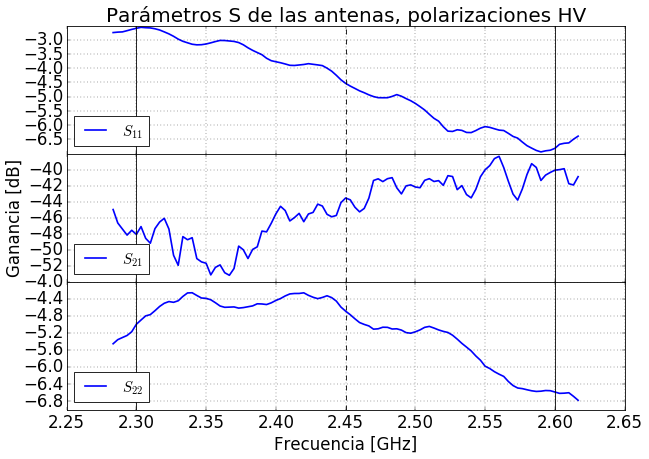
\includegraphics[width=7cm]{SParamsHV}
    \caption{Polarización HV}
    \label{subfig:hvPol}
  \end{subfigure}

  \begin{subfigure}{0.47\textwidth}
    \centering
    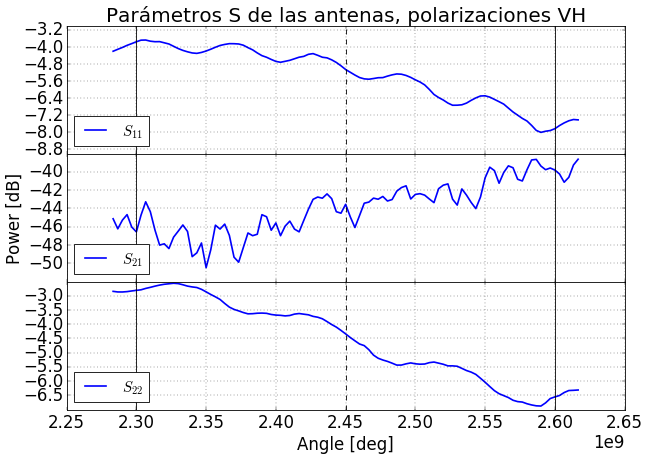
\includegraphics[width=7cm]{SParamsVH}
    \caption{Polarización VH}
    \label{subfig:vhPol}
  \end{subfigure}
  \begin{subfigure}{0.47\textwidth}
    \centering
    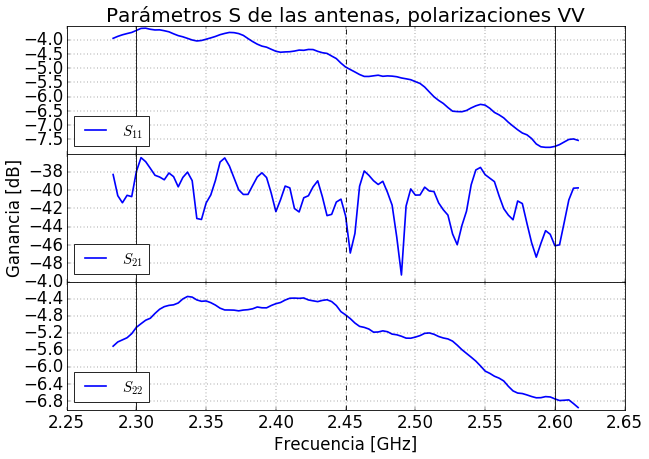
\includegraphics[width=7cm]{SParamsVV}
    \caption{Polarización VV}
    \label{subfig:vvPol}
  \end{subfigure}
  \caption{Mediciones de parámetros S de las antenas en todas las combinaciones de polarizaciones. \ref{subfig:hhPol} HH, \ref{subfig:hvPol} HV, \ref{subfig:vhPol} VH y \ref{subfig:vvPol} VV.}
  \label{fig:sParametersMeasurements}
\end{figure}

Se puede apreciar que si bien los coeficientes de reflexión son similares entre polarizaciones, todos muestran una gran variación de respuesta a lo largo de la frecuencia de trabajo, llegando a ser de hasta $\SI{4.6}{\dB}$. Por el lado de la variación del coeficiente de transmisión, la polarización HH solamente está en el orden de los $\SI{4.5}{\dB}$. En cambio para el resto de las polarizaciones, la misma resulta ser del orden de los $\SI{12}{\dB}$.

La tabla \ref{tab:antennasParameters} resume los valores medidos de cada parámetros S a la frecuencia central. Se puede apreciar que los coeficientes de reflexión de cada antena en cada polarización permanece invariante ante las combinaciones de polarizaciones utilizadas. A su vez, se puede apreciar que el coeficiente de transmisión directo permanece casi igual al coeficiente de transmisión inverso y que dichos coeficientes también son iguales entre las polarizaciones HV y VH. Por último, cabe destacar que las polarizaciones HH poseen un mayor coeficiente de transmisión que las VV en un orden de $\SI{8}{\dB}$.

\begin{table}[htb]
  \caption{Parámetros S de las antenas medidos con un VNA a frecuencia central.}
  \centering
  \label{tab:antennasParameters}
  \begin{tabular}{l *{4}{S[table-auto-round, table-format=-2.2]}}
  \toprule
  \multirow{2}{*}{\textbf{Parámetro S}} & \multicolumn{4}{c}{\textbf{Polarizaciones}} \tabularnewline
  \cmidrule{2-5}
  & HH & HV & VH & VV \tabularnewline
  \midrule
  
  $S_{11}$ & -4.46033873376335 & -4.53492363950625 & -5.06302223793916 & -4.95964466600015 \tabularnewline

  $S_{12}$ & -34.8204780020621 & -43.4389116307712 & -43.5577358595805 & -42.7387139376128 \tabularnewline

  $S_{21}$ & -34.7141043352772 & -43.5629806134325 & -43.4259094492972 & -42.8482094658858 \tabularnewline

  $S_{22}$ & -4.32197124367156 & -4.69545953806287 & -4.34205880309025 & -4.78356133012197 \tabularnewline

  \bottomrule
  \end{tabular}
\end{table}


\subsection{Diagrama de Radiación}

Para esta medición se desconectó del radar la antena receptora y se la conectó en el analizador de espectros a una distancia igual a $\SI{1.427}{\meter}$ para medir la potencia recibida por el radar, ver figura \ref{fig:radiationPatternConnections}. A la antena transmisora se la fue rotando a medida que se tomaban muestras para obtener el diagrama de radiación. Por último, tanto a la antena transmisora como la receptora se le fueron cambiando las polarizaciones para obtener el diagrama en todas las posibles combinaciones, HH, HV, VH y VV.
\begin{figure}[htb]
 \centering
 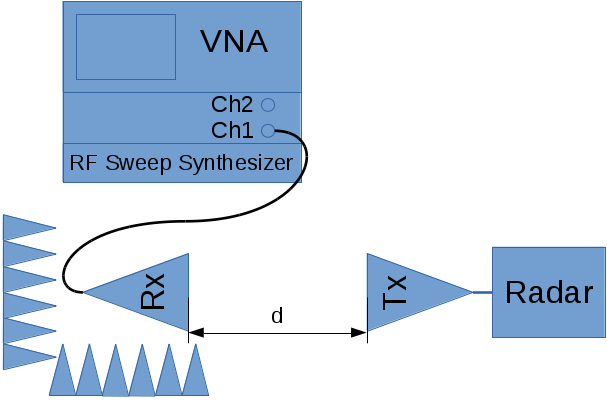
\includegraphics[width=8cm]{RadiatingPatternAntenaWorkbench}
 \caption{Banco de medición, diagrama de radiación entre antenas.}
 \label{fig:radiationPatternConnections}
\end{figure}

Es importante notar en la imagen \ref{fig:radiationPatternConnections} que la antena receptora se la colocó frente a absorbedores para disminuir la potencia recibida proveniente de ecos en las paredes de la sala en que se realizó la medición. La tabla \ref{tab:PNAConfigRadiationPattern} resume las configuraciones utilizadas en el analizador de espectros para las mediciones.

\begin{table}[H]
  \caption{Configuración del analizador de espectros, medición del diagrama de radiación.}
  \centering
  \label{tab:PNAConfigRadiationPattern}
  \begin{tabular}{l c c}
  \toprule
  \textbf{Característica} & \textbf{Configuración} & \textbf{Unidad} \tabularnewline
  \midrule
  Mode & ANALYZER & \tabularnewline

  Center Freq & 2434262820,514000 & \si{\hertz} \tabularnewline

  Freq Offset & 0,000000 & \si{\hertz} \tabularnewline

  Span & 100000000,000000 & \si{\hertz} \tabularnewline

  x-Axis & LIN & \tabularnewline

  Start & 2384262820,514000 & \si{\hertz} \tabularnewline

  Stop & 2484262820,514000 & \si{\hertz} \tabularnewline

  Ref Level & -9,000000 & \si{\dBm} \tabularnewline

  Level Offset & 0,000000 & \si{\dB} \tabularnewline

  Ref Position & 100,000000 & \si{\percent} \tabularnewline

  y-Axis & LOG & \tabularnewline

  Level Range & 100,000000 & \si{\dB} \tabularnewline

  Rf Att & 5,000000 & \si{\dB} \tabularnewline

  RBW & 2000000,000000 & \si{\hertz} \tabularnewline

  VBW & 50,000000 & \si{\hertz} \tabularnewline

  SWT & 2,500000 & \si{\second} \tabularnewline

  Trace Mode & CLR/WRITE & \tabularnewline

  Detector & RMS & \tabularnewline

  Sweep Count & 0 & \tabularnewline
  \bottomrule
  \end{tabular}
\end{table}

La tabla \ref{tab:antennaPattern} resume los resultados de las mediciones realizadas y la imagen \ref{fig:patterns} muestra los diagramas de radiación. Se puede observar que el ancho del lóbulo principal para las polarizaciones HH y VV son muy similares, aproximadamente de unos $\SI{50}{\degree}$ y que las ganancias máximas del mismo rondan los $\SI{-22}{\dB}$. En cambio, se nota que para HH los lóbulos secundarios son $\SI{3}{\dB}$ mayores y los mismos se encuentran a $\SI{3.8}{\dBc}$ para HH y $\SI{6.55}{\dBc}$ para VV.

Por último, comparando los gráficos co-polares con respecto al cross-polar, se puede observar que el rechazo por polarización cruzada es de $\SI{18}{\dB}$, dado que la ganancia recibida es de $\SI{-40}{\dB}$ frente a los $\SI{-22}{\dB}$ de las co-polares, para el centro del lóbulo principal. A su vez se observa que los lóbulos secundarios poseen una ganancia mayor, llegando a los $\SI{-37}{\dB}$.

\begin{figure}
  \centering
  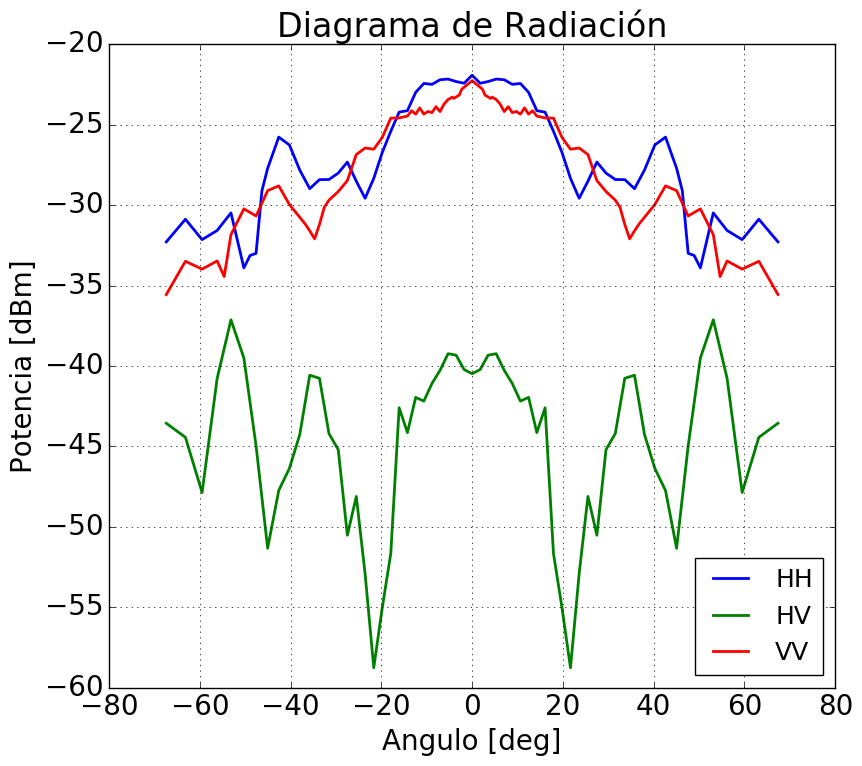
\includegraphics[width=10cm]{patterns}
  \caption{Diagrama de radiación del radar en distintas combinaciones de polarizaciones, HH, HV y VV.}
  \label{fig:patterns}
\end{figure}

\begin{table}[H]
  \caption{Mediciones diagrama de radiación entre polarizaciones.}
  \centering
  \label{tab:antennaPattern}
  \begin{tabular}{*{5}{S[table-auto-round, table-format=-2.2]}}
  \toprule
  \multirow{2}{*}{\textbf{ángulos entre antenas [$\si{\degree}$]}} & \multicolumn{4}{c}{\textbf{Potencia transmitida en polarizaciones}} \tabularnewline
  \cmidrule{2-5}
   & HH & HV & VH & VV \tabularnewline
  \midrule
  0.0 & -21.914052963256836 & -40.480464935302734 & -40.480464935302734 & -22.251615524291992 \tabularnewline

  1.91021317171 & -22.4134578704834 & -40.224273681640625 & -40.224273681640625 & -22.784189224243164 \tabularnewline

  3.82255372927 & -22.30802345275879 & -39.3284797668457 & -39.3284797668457 & -23.145263671875 \tabularnewline

  5.73917047727 & -22.154735565185547 & -39.235477447509766 & -39.235477447509766 & -23.423660278320312 \tabularnewline

  7.66225566077 & -22.194988250732422 & -40.26947021484375 & -40.26947021484375 & -24.174240112304688 \tabularnewline

  9.59406822686 & -22.48287582397461 & -41.09086608886719 & -41.09086608886719 & -24.239660263061523 \tabularnewline

  11.5369590328 & -22.42629051208496 & -42.18770980834961 & -42.18770980834961 & -24.336830139160156 \tabularnewline

  13.4933988216 & -22.981735229492188 & -41.95241928100586 & -41.95241928100586 & -24.332292556762695 \tabularnewline

  15.4660099534 & -24.11693000793457 & -44.143924713134766 & -44.143924713134766 & -24.45547866821289 \tabularnewline

  17.4576031237 & -24.21193504333496 & -42.601112365722656 & -42.601112365722656 & -24.572660446166992 \tabularnewline

  19.4712206345 & -25.39852523803711 & -51.66230010986328 & -51.66230010986328 & -24.58316993713379 \tabularnewline

  21.5101882669 & -26.707298278808594 & -55.01024627685547 & -55.01024627685547 & -25.775318145751953 \tabularnewline

  23.5781784782 & -28.32943344116211 & -58.773075103759766 & -58.773075103759766 & -26.516315460205078 \tabularnewline

  25.6792886195 & -29.568967819213867 & -52.928672790527344 & -52.928672790527344 & -26.44162368774414 \tabularnewline

  27.8181392847 & -28.507495880126953 & -48.11441421508789 & -48.11441421508789 & -26.84745216369629 \tabularnewline

  30.0 & -27.317434310913086 & -50.52842330932617 & -50.52842330932617 & -28.46544075012207 \tabularnewline

  32.2309526355 & -28.002696990966797 & -45.20555877685547 & -45.20555877685547 & -29.152206420898438 \tabularnewline

  34.5181078411 & -28.401615142822266 & -44.20515060424805 & -44.20515060424805 & -29.684959411621094 \tabularnewline

  36.8698976458 & -28.40848731994629 & -40.76640701293945 & -40.76640701293945 & -31.19536590576172 \tabularnewline

  39.2964802392 & -28.97147560119629 & -40.5757942199707 & -40.5757942199707 & -31.591350555419922 \tabularnewline

  41.8103148958 & -27.810001373291016 & -44.27327346801758 & -44.27327346801758 & -30.774405479 \tabularnewline

  44.4270040008 & -26.254615783691406 & -46.36780548095703 & -46.36780548095703 & -29.957460403442383 \tabularnewline

  47.1665719339 & -25.764413833618164 & -47.74458694458008 & -47.74458694458008 & -28.79700469970703 \tabularnewline

  50.0554948102 & -27.705350875854492 & -51.336891174316406 & -51.336891174316406 & -29.092802047729492 \tabularnewline

  53.1301023542 & -32.99269104003906 & -44.96973419189453 & -44.96973419189453 & -30.67097282409668 \tabularnewline

  56.4426902381 & -33.899192810058594 & -39.50574493408203 & -39.50574493408203 & -30.22670555114746 \tabularnewline

  60.0735651334 & -30.478853225708008 & -37.128719329833984 & -37.128719329833984 & -31.830547332763672 \tabularnewline

  64.1580672368 & -31.572757720947266 & -40.781593322753906 & -40.781593322753906 & -33.468048095703125 \tabularnewline

  68.9605302187 & -32.14019012451172 & -47.87135314941406 & -47.87135314941406 & -33.976505279541016 \tabularnewline

  75.164888418 & -30.873291015625 & -44.438751220703125 & -44.438751220703125 & -33.48764419555664 \tabularnewline

  90.0 & -32.28058624267578 & -43.56352233886719 & -43.56352233886719 & -35.55542755126953 \tabularnewline
  \bottomrule
  \end{tabular}
\end{table}


\section{Resumen}

En este capítulo se detallaron todos los subsistemas de hardware que componen al radar. Los mismos son el modulador, la cadena de RF, las antenas transmisoras y receptoras, el filtro pasa bajos y por último el gabinete. A su vez se midió cada uno de los mismos para verificar su correcto funcionamiento y cumplimiento de los requerimientos de nivel 2.

El circuito modulador fue construido de tal forma de poder transmitir más de un tipo de modulación ante la posibilidad de realizar futuros ensayos con distintos tipos de señales transmitidas, requerimiento \ref{req:l2_mod}. Las posibles modulaciones son diente de sierra creciente o decreciente, triangular y sinusoidal.

La potencia transmitida por la cadena de RF sin modular es igual a $\SI{1.87}{\dBm}$, al modular con el diente de sierra se obtiene un ancho de banda igual a $\SI{291.67}{\MHz}$.

Tanto para aumentar la directividad de las antenas como para que cada una sea polarimétrica, se hace uso de cavidades, que por simplicidad son cilíndricas. En un paso futuro, para asegurar la polarimetría se deben utilizar prismas rectangulares y para disminuir el cross-talk entre polarizaciones de una misma antena, se debe separar cada monopolo en una longitud de onda. Con respecto a las mediciones de comportamiento de las antenas, se puede observar que el coeficiente de reflexión de ronda los $\SI{-5}{\dB}$ y que los coeficientes de transmisión entre polarizaciones ronda los $\SI{-43}{\dB}$ salvo para HH que ronda los $\SI{-35}{\dB}$.

Por último, se midió el diagrama de radiación a una distancia de $\SI{1.427}{\meter}$, se puede determinar que el rechazo de polarización cruzada es de $\SI{18}{\dB}$ siendo la ganancia recibida del centro del lóbulo principal para el caso co-polar igual a $\SI{-22}{\dB}$. Por último, los lóbulos secundarios se encuentran a $\SI{50}{\degree}$ y los mismos poseen una potencia de $\SI{3.8}{\dBc}$ para el caso HH y de $\SI{6.55}{\dBc}$ para el caso VV.
